\PassOptionsToPackage{unicode=true}{hyperref} % options for packages loaded elsewhere
\PassOptionsToPackage{hyphens}{url}
\PassOptionsToPackage{dvipsnames,svgnames*,x11names*}{xcolor}
%
\documentclass[16pt,]{krantz}
\usepackage{lmodern}
\usepackage{amssymb,amsmath}
\usepackage{ifxetex,ifluatex}
\usepackage{fixltx2e} % provides \textsubscript
\ifnum 0\ifxetex 1\fi\ifluatex 1\fi=0 % if pdftex
  \usepackage[T1]{fontenc}
  \usepackage[utf8]{inputenc}
  \usepackage{textcomp} % provides euro and other symbols
\else % if luatex or xelatex
  \usepackage{unicode-math}
  \defaultfontfeatures{Ligatures=TeX,Scale=MatchLowercase}
    \setmonofont[Mapping=tex-ansi,Scale=0.7]{Source Code Pro}
\fi
% use upquote if available, for straight quotes in verbatim environments
\IfFileExists{upquote.sty}{\usepackage{upquote}}{}
% use microtype if available
\IfFileExists{microtype.sty}{%
\usepackage[]{microtype}
\UseMicrotypeSet[protrusion]{basicmath} % disable protrusion for tt fonts
}{}
\IfFileExists{parskip.sty}{%
\usepackage{parskip}
}{% else
\setlength{\parindent}{0pt}
\setlength{\parskip}{6pt plus 2pt minus 1pt}
}
\usepackage{xcolor}
\usepackage{hyperref}
\hypersetup{
            pdftitle={Morfología visual},
            pdfauthor={Ricardo Michel MALLQUI BAÑOS},
            colorlinks=true,
            linkcolor=Maroon,
            filecolor=Maroon,
            citecolor=Blue,
            urlcolor=Blue,
            breaklinks=true}
\urlstyle{same}  % don't use monospace font for urls
\usepackage{longtable,booktabs}
% Fix footnotes in tables (requires footnote package)
\IfFileExists{footnote.sty}{\usepackage{footnote}\makesavenoteenv{longtable}}{}
\setlength{\emergencystretch}{3em}  % prevent overfull lines
\providecommand{\tightlist}{%
  \setlength{\itemsep}{0pt}\setlength{\parskip}{0pt}}
\setcounter{secnumdepth}{5}

% set default figure placement to htbp
\makeatletter
\def\fps@figure{htbp}
\makeatother

\usepackage[spanish,es-lcroman]{babel}
\usepackage{booktabs}
\usepackage{mathtools}
\usepackage{graphicx}
\usepackage{amsmath}
\usepackage{makeidx}
\makeindex
%\usepackage{showframe}
%\usepackage[a4paper]{geometry}
%\geometry{verbose,tmargin=3cm,bmargin=3cm,lmargin=3.5cm,rmargin=3cm}
\setlength\parindent{23pt}
\usepackage[singlelinecheck=off]{caption}

\usepackage{times}
\renewcommand{\rmdefault}{ptm}
%\usepackage[lite,subscriptcorrection,nofontinfo,zswash]{mtpro2}

\usepackage{graphicx}

% Determine if the image is too wide for the page.
\makeatletter
\def\ScaleIfNeeded{%
  \ifdim\Gin@nat@width>\linewidth
    \linewidth
  \else
    \Gin@nat@width
  \fi
}
\makeatother

% Resize figures that are too wide for the page.
%\let\oldincludegraphics\includegraphics
%\renewcommand\includegraphics[2][]{%
%  \oldincludegraphics[scale=0.85]{#2}
%}

\usepackage{amsthm}
\makeatletter
\def\thm@space@setup{%
  \thm@preskip=8pt plus 2pt minus 4pt
  \thm@postskip=\thm@preskip
}
\makeatother

\flushbottom 

\frontmatter
\usepackage[]{natbib}
\bibliographystyle{apalike}

\title{Morfología visual}
\author{Ricardo Michel MALLQUI BAÑOS}
\providecommand{\institute}[1]{}
\institute{Universidad Nacional San Cristóbal De Huamanga}
\date{2021-07-16}

\usepackage{amsthm}
\newtheorem{theorem}{Teorema}[chapter]
\newtheorem{lemma}{Lema}[chapter]
\newtheorem{corollary}{Corolario}[chapter]
\newtheorem{proposition}{Proposición}[chapter]
\newtheorem{conjecture}{Conjectura}[chapter]
\theoremstyle{definition}
\newtheorem{definition}{Definición}[chapter]
\theoremstyle{definition}
\newtheorem{example}{Ejemplo}[chapter]
\theoremstyle{definition}
\newtheorem{exercise}{Ejercicio}[chapter]
\theoremstyle{definition}
\newtheorem{hypothesis}{Hypothesis}[chapter]
\theoremstyle{remark}
\newtheorem*{remark}{Observación}
\newtheorem*{solution}{Solución}
\begin{document}
\maketitle

%\cleardoublepage\newpage\thispagestyle{empty}\null
%\cleardoublepage\newpage\thispagestyle{empty}\null
%\cleardoublepage\newpage
\thispagestyle{empty}
\begin{flushright}
Universidad Nacional San Cristobal de Huamanga

Fisart.cf

Agradecimento a los estudiantes de la ESFAPA FGPA

A la UNSCH

\includegraphics[height=3cm]{U.pdf}
\end{flushright}
%\setlength{\abovedisplayskip}{-5pt}
%\setlength{\abovedisplayshortskip}{-5pt}

{
\hypersetup{linkcolor=}
\setcounter{tocdepth}{2}
\tableofcontents
}
\listoftables
\listoffigures
\newcommand{\N}{\mathbb{N}}
\newcommand{\R}{\mathbb{R}}
\newcommand{\CC}{\mathbb{C}}
\newcommand{\I}{\mathbb{I}}
\newcommand{\f}{\mathbb{f}}
\newcommand{\X}{\mathbb{X}}
\newcommand{\D}{\mathbb{D}}
\newcommand{\Z}{\mathbb{Z}}
\newcommand{\Q}{\mathbb{Q}}
\newcommand{\norm}[1]{\left\Vert#1\right\Vert}
\newcommand{\abs}[1]{\left\vert#1\right\vert}
\newcommand{\set}[1]{\left\{#1\right\}}
\newcommand{\seq}[1]{\left<#1\right>}
\newcommand{\co}[1]{\left[#1\right]}
\newcommand{\cc}[1]{\left(#1\right)}
\newcommand{\J}{\mathcal{J}}
\newcommand{\K}{\mathcal{K}}
\newcommand{\M}{\mathcal{M}}
\newcommand{\F}{\mathcal{F}}

\hypertarget{resumen}{%
\chapter*{Resumen}\label{resumen}}


La importancia del estudio de la forma en el arte plástico se debe a la manipulación constante de estas en el espacio bidimensional y tridimensional. En el plano bidimensional se estudian aspectos geometricos partiendo desde la forma de un punto hasta formas orgánicas con comportamientos similares al de los conjuntos fractales de Mandelbrot y Julia y en el espacio tridimensional se realiza un estudio sobre formas que viven en este espacio es decir tanto las formas bidimensionales además de los sólidos geométricos y las formas orgánicas y los conjuntos fractales de Mandelbrots 3D y julia 3D. Finalmente se realiza composiciones con estas formas, utilizando principios de composicon plástica con el objetivo de reunir los conocimientos previos y reconocer la utilidad de su estudio previo. Luego se reconocerán estas formas como contenedores de formas existentes en la naturaleza tales como las formas estudiadas en la fitomorfología, la zoomorfología, la geomorfologia. En el Apendice se describen conceptos relacionados a transformaciones y centros de masa de formas 2d y 3d.

\hypertarget{introducciuxf3n}{%
\chapter*{Introducción}\label{introducciuxf3n}}


El estudio de la forma de manera aislada o compositiva, en el arte plástico es de importancia para la manipulación correcta de estas, generando representación lógica; es decir desprovista de la intuición, la intuición, generalmente distorsiona el aspecto verdadero de las formas.

El espacio bidimensional se denota con el símbolo \(\mathbb{R}^2\) y al espacio tridimensional se denota con el símbolo \(\mathbb{R}^3\). Las formas bidimensionales pueden existir tanto el el espacio bidimensional y tridimensional y Las formas tridimensionales únicamente pueden se representados en el espacio tridimensional.

Las formas que reunen todas las caracteristicas de las formas bidimensionales y tridimensionales son los las formas llamadas fractales tridimensionales que se generan bajo procesos de iteración o recursividad de transformaciones de las copias de ciertas formas básicas llamadas módulos, exiten modelos secuenciales que indican la recursividad, la formas concernientes a los fractales generadas por los números complejos son las llamadas conjuntos de Mandelbrot y Julia en el espacio bidimensional y el el espacio tridimensional se llaman conjuntos de Mandelbrot 3D y Julia 3D, estas formas manifiestan una variedad infinita.

El libro se realiza bajo las teorías y conceptos de diversas áreas tales como la botánica la geometría descriptiva, modelos matemáticos, que proveen de conceptos y objetos utilizados hasta el momento de manera intuitiva en las artes plásticas es decir se interrelaciona estos conocimientos con el objetivo de agruparlos de manera lógica y secuencial, avalada evidentemente por las teorías y la intuición genuina.

Las formas orgánicas son aquellas que escapan a una geometría especifica ya estudiadas pero pueden ser estudiadas bajo criterios de geometrización es decir generando una red geométrica que lo inscriban, esto es identificando los puntos sobre la forma que sirvan de anclaje o vértice, estos puntos pueden pertenecer o no la forma en el primer caso se debe considerar que sean puntos más resaltantes de la forma, en el segundo caso deben ser punto de manera que generan segmentos tangentes a la forma considerada.

El libro se compone de cinco capítulos en los cuales se describen los temas de manera secuencial además de dos apéndices que sirven como reforzamiento de la ideas vertidas en el texto es decir en el primer capitulo se describe la teoría de la forma en el espacio bidimensional, en el capitulo 2 se describe la teoría de las formas tridimensionales, en el tercer capítulo concierne a la teoría de formas compositivas, el capítulo 4 formas orgánicas y su geometría, el capítulo 5 formas abstractas y su geometría.

\mainmatter

\hypertarget{formas-bidimesionales}{%
\chapter{Formas bidimesionales}\label{formas-bidimesionales}}

En este capítulo se describirán definiciones y conceptos sobre las \emph{formas básicas} que pueden ser representadas en el \emph{espacio bidimensional} \index{espacio bidimensional} \(\mathbb{R}^2\) tales como el punto, la linea, los polígonos, las formas orgánicas y los fractales bidimensionales.

\hypertarget{el-punto-y-la-linea}{%
\section{El punto y la linea}\label{el-punto-y-la-linea}}

Primeramente definamos el \emph{espacio} donde se manipularán las \emph{formas bidimensionales}, la importancia de este espacio se debe a la necesidad de un \emph{sistema de referencia}\index{sistema de referencia} que deben tener los objetos tales como la ubicación, la dirección, la relación de dos o más objetos entre otros.

\begin{definition}[ Espacio bidimesional]
\protect\hypertarget{def:r2}{}{\label{def:r2} \iffalse ( Espacio bidimesional) \fi{} }
\end{definition}

El espacio bidimensional \index{espacio bidimensional} es un \emph{conjunto de puntos,} \index{conjunto de puntos} donde cada punto utiliza como su \emph{sistema de referencia} a un \emph{par de rectas} \emph{llamadas ejes}, la primera recta es \emph{horizontal} \index{horizontal} llamada ``eje \(x\)'' y la otra es \emph{vertical} \index{vertical} llamada ``eje \(y\)''.

\begin{figure}[!ht]

{\centering 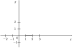
\includegraphics{ejes} 

}

\caption{Sistema de ejes coordenados}\label{fig:2d}
\end{figure}

Estos ejes \textbf{\emph{evidentemente}} se \emph{interceptan} en un punto, formando cuatro ángulos iguales a \(90^\circ\) es decir son \textbf{\emph{perpendiculares}}, y cuatro regiones llamadas cuadrantes. Ademas la intersección de los ejes indica la posición cero; siendo la numeración hacia la derecha del eje \(x\) y hacia arriba del eje \(y\) positiva, además hacia la izquierda del eje \(x\) y hacia abajo del eje \(y\), negativa. En los ejes podemos ubicar a los números reales e irracionales; refiérase a la Figura \ref{fig:2d}.

\begin{remark}
\iffalse{} {Observación. } \fi{}Existen otros términos que refieren al espacio bidimensional, por ejemplo a veces suele llamarse como plano, sistema de ejes coordenados 2d o simplemente como el espacio 2d.
\end{remark}

\begin{definition}[El punto]
\protect\hypertarget{def:punto}{}{\label{def:punto} \iffalse (El punto) \fi{} }El punto es un ente grafico, considerada como la mínima unidad en la representacion gráfica. Refiérase a la Figura (\ref{fig:puntolinea})
\end{definition}

\begin{figure}[!ht]

{\centering 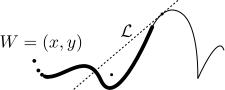
\includegraphics{puntolinea} 

}

\caption{El punto y la linea (magnificada)}\label{fig:puntolinea}
\end{figure}

La ubicación de un punto se realiza con la ayuda de un sistema de ejes coordenados refiérase a la Definición \ref{def:r2} compuestas de dos ejes el eje \(x\) (eje de las abscisas) y el eje \(y\) (eje de las ordenadas), ademas de una etiqueta de ser necesaria, es decir el punto \(W=(x,y)\) (etiquetas con letras mayúsculas), indica que esta ubicada a \(x\) unidades sobre el eje \(x\), del centro del sistema de ejes coordenados, a la derecha si \(x\) es positivo y a la iquierda si \(x\) es negativo; y \(y\) unidades sobre el eje \(y\), del centro del sistema de ejes coordenados, hacia arriba si \(y\) es positivo y hacia abajo si \(y\) es negativo.

\begin{definition}[La linea]
\protect\hypertarget{def:linea}{}{\label{def:linea} \iffalse (La linea) \fi{} }La linea considerada como el conjunto de puntos distribuidas de manera secuencial es decir yuxtapuestas. Refiérase a la Figura (\ref{fig:puntolinea})
\end{definition}

Para la clasificación de las lineas es necesario considerar algunas definiciones previas por ejemplo la \emph{dirección de una linea} en un punto dado y el \emph{punto vértice}.

\begin{definition}[Dirección de una recta]
\protect\hypertarget{def:direccionrecta}{}{\label{def:direccionrecta} \iffalse (Dirección de una recta) \fi{} }La dirección de un recta es la inclinación con respecto a una linea horizontal (eje \(x\)) medida en angulos, con grados sexagesimales en sentido antihorario.
\end{definition}

Por ejemplo en la Figura \ref{fig:tangente} se tiene que la \emph{pendiente} de las dos rectas punteada están definidas por las inclinaciones de \(\alpha\) y \(\beta\) con respecto a un linea horizontal, es decir las pendientes son las tangentes de estos ángulos esto es \(\tan \alpha\) y \(\tan \beta\) respectivamente. Además se puede observar que la pendiente de la recta cuyo ángulo de inclinación \(\alpha\) es mayor a la pendiente de la recta cuya inclinación es de \(\beta\). Recuérdese que los ángulos considerados son los sexagesimales, aunque no es restrictiva.

Las rectas verticales tienen una inclinación de \(90^\circ\) o múltiplos de esta, es decir la pendiente es \(\tan 90^\circ=\infty\) y las rectas horizontales tienen una inclinación de \(0^\circ\) o multiplos de esta, por tanto la pendiente es \(\tan 0^\circ=0\).

\begin{definition}[Recta tangente]
\protect\hypertarget{def:tangentew}{}{\label{def:tangentew} \iffalse (Recta tangente) \fi{} }Es un \emph{recta} asociada a una \emph{linea} en un punto determinado, si estas comparten unicamente dicho punto en una vecindad pequeña de esta.
\end{definition}

Por ejemplo la linea \(\mathcal{L}\) la Figura \ref{fig:tangente} es una \emph{recta tangente} en el punto \(W'\) pues esta recta tiene intersección con la curva \(GW\) únicamente en el punto \(W'\) en una vecindad muy pequeña de \(W'\).

\begin{definition}[Dirección de una linea en un punto]
\protect\hypertarget{def:direccion}{}{\label{def:direccion} \iffalse (Dirección de una linea en un punto) \fi{} }La dirección de un linea en un punto esta definida por la direccion de la \emph{recta tangente} en el punto considerado.
\end{definition}

En la Figura \ref{fig:tangente} se tiene la dirección de la linea en el punto \(W'\) definida por la pendiente de la recta tangente en dicho punto.

Debido a la igualdad de las direcciones en los puntos de una linea recta la dirección de una recta o un segmento se considera como única es decir el segmento o la recta son las tangentes a las mismas por tanto la pendiente son las pendientes del segmento o recta considera.

\begin{definition}[Punto vértice]
\protect\hypertarget{def:puntovertice}{}{\label{def:puntovertice} \iffalse (Punto vértice) \fi{} }Un vertice es un punto de una linea, donde en una vecindad pequeña del punto cambia de direccion en los puntos adyacentes, es decir la tangente cambia drasticamente a la izquierda y derecha del punto.
\end{definition}

\begin{figure}[!ht]

{\centering 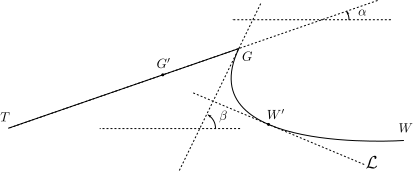
\includegraphics{tangente} 

}

\caption{El punto vértice y dirección puntual}\label{fig:tangente}
\end{figure}

Las lineas se pueden clasificar de acuerdo al comportamiento de uno o más de sus puntos, es decir un punto además de ser parte de una linea podría tener la característica adicional de ser un punto vértice, refiérase a la Definición \ref{def:puntovertice}. Existen tres clases de lineas:

\begin{enumerate}
\def\labelenumi{\arabic{enumi}.}
\item
  Lineas curvas.
\item
  Lineas rectas -------

  \begin{itemize}
  \tightlist
  \item
    Rectas
  \item
    Segmentos
  \end{itemize}
\item
  Lineas mixtas
\end{enumerate}

Si una linea no presenta puntos vértices entonces la linea simplemente es una curva liza y continua (sin picos), es decir una \textbf{linea curva}. Las lineas rectas\ldots{} cuya \emph{longitud es finita} recibe el nombre de \textbf{segmento} y si la \emph{longitud es infinita} recibe el nombre de \textbf{recta\ldots{}}; ademas la lineas mixtas son generadas por la unión de lineas \emph{curvas} y \emph{rectas\ldots{}} presentando puntos vértice en las conexiones entre ellas.

Además en la Figura \ref{fig:tangente} se tiene que la linea \(GW\) es una curva, la linea \(TG\) es una linea recta en particular un segmento y la linea \(TGW\) es un \textbf{linea mixta} pues es la union de las lineas \(TG\) y \(GW\).

\hypertarget{poluxedgonales}{%
\section{Polígonales}\label{poluxedgonales}}

Las lineas poligonales generan formas poligonales\index{poligonales} que son \emph{lineas mixtas} generadas por la \emph{unión segmentos} de longitudes iguales o diferentes. Existen formas poligonales abiertas y cerradas regulares e irregulares que tienen la utilidad de en el arte de diversas índole.

\begin{definition}
\protect\hypertarget{def:poligonal}{}{\label{def:poligonal} }Las lineas poligonales son fornas obtenidas mediante la unión consecutiva de segmentos con direcciones distintas.
\end{definition}

\begin{figure}[!ht]

{\centering 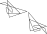
\includegraphics{simetria} 

}

\caption{Simetria}\label{fig:simetria}
\end{figure}

\hypertarget{poligonales-abiertos}{%
\subsection{Poligonales abiertos}\label{poligonales-abiertos}}

Estas lineas poligonales no encierran ninguna región, es decir el extremo final del ultimo segmento no coincide con el extremo inicial del primer segmento.

\begin{definition}[Linea poligonal]
\protect\hypertarget{def:poligono}{}{\label{def:poligono} \iffalse (Linea poligonal) \fi{} }La linea considerada como el conjunto de puntos distribuidas de manera secuencial es decir yuxtapuestas. Observe la figura (\ref{fig:2d}).
\end{definition}

\hypertarget{poligonales-cerrados}{%
\subsection{Poligonales cerrados}\label{poligonales-cerrados}}

Son aquellas que encierran una región en el plano bidimensional, es decir dividen el plano bidimensional en dos regiones una limitada y la otra ilimitada. Además el extremo final del ultimo segmento coincide con el extremo inicial del primer segmento.

\hypertarget{irregulares}{%
\subsubsection{Irregulares}\label{irregulares}}

\begin{definition}[Polígonos rregulares]
\protect\hypertarget{def:irregulares}{}{\label{def:irregulares} \iffalse (Polígonos rregulares) \fi{} }La linea considerada como el conjunto de puntos distribuidas de manera secuencial es decir yuxtapuestas. Observe la figura (\ref{fig:2d}).
\end{definition}

\hypertarget{regulares}{%
\subsubsection{Regulares}\label{regulares}}

\begin{definition}[Polígonos irregulares]
\protect\hypertarget{def:regulares}{}{\label{def:regulares} \iffalse (Polígonos irregulares) \fi{} }La linea considerada como el conjunto de puntos distribuidas de manera secuencial es decir yuxtapuestas. Observe la figura (\ref{fig:2d}).
\end{definition}

Refiérase al cuadro \ref{tab:regulares}

\begin{longtable}[]{@{}cccc@{}}
\caption{\label{tab:regulares} Polígonos cerrados regulares.}\tabularnewline
\toprule
Tipo & Número de lados & Número de diagonales & Apotemas\tabularnewline
\midrule
\endfirsthead
\toprule
Tipo & Número de lados & Número de diagonales & Apotemas\tabularnewline
\midrule
\endhead
Triángulo equilátero & 3 & 0 & 3\tabularnewline
Cuadrado & 4 & 2 & 4\tabularnewline
Pentágono & 5 & 5 & 5\tabularnewline
Exagono & 6 & 6 & 6\tabularnewline
Heptagono & 7 & 7 & 7\tabularnewline
\ldots{} & \ldots{} & \ldots{} & \ldots{}\tabularnewline
\bottomrule
\end{longtable}

\begin{longtable}[]{@{}lll@{}}
\caption{\label{tab:regular} WWWWWW}\tabularnewline
\toprule
Col1 & Col2 & Col3\tabularnewline
\midrule
\endfirsthead
\toprule
Col1 & Col2 & Col3\tabularnewline
\midrule
\endhead
w & w & w\tabularnewline
w & w & w\tabularnewline
w & w & ww\tabularnewline
\bottomrule
\end{longtable}

\hypertarget{curvas-cerradas}{%
\section{Curvas cerradas}\label{curvas-cerradas}}

Similar al caso de los poligonos cerrados estas formas generan dos regiones en el plano bidimensional una en el interior de esta forma y otra en el exterior.

\hypertarget{la-circunferencia}{%
\subsection{La circunferencia}\label{la-circunferencia}}

\begin{definition}[La circunferencia]
\protect\hypertarget{def:circulo}{}{\label{def:circulo} \iffalse (La circunferencia) \fi{} }Es la curva geenrada por los puntos que equidistan de un punto llamado centro de la cirunferencia
\end{definition}

\hypertarget{la-elipse}{%
\subsection{La elipse}\label{la-elipse}}

\begin{definition}[Elipse]
\protect\hypertarget{def:elipse}{}{\label{def:elipse} \iffalse (Elipse) \fi{} }wwwwwwwwwwwwwwwwwwwwwwwwwwww
\end{definition}

\hypertarget{trasformaciuxf3n-de-la-elipse}{%
\subsection{Trasformación de la elipse}\label{trasformaciuxf3n-de-la-elipse}}

\hypertarget{lugares-geomuxe9tricos}{%
\section{Lugares geométricos}\label{lugares-geomuxe9tricos}}

LOs lugares geoemétricos son formas que se obtiene mediante el movimiento de uno o más puntos restringidos a un sistema de referencia de longitud y ángulo.

\hypertarget{las-cuxf3nicas}{%
\subsection{Las cónicas}\label{las-cuxf3nicas}}

\hypertarget{otros}{%
\subsection{Otros\ldots{}}\label{otros}}

\hypertarget{fractales-bidimesionales}{%
\section{Fractales bidimesionales}\label{fractales-bidimesionales}}

Los fractales son objetos cuya estructura esta basada en suceción de formas ademas de las transformaciones elementales refiérase al apéndice.

\hypertarget{fractales-cluxe1sicos}{%
\subsection{Fractales clásicos}\label{fractales-cluxe1sicos}}

\begin{definition}[Triangulos de Sierpinski]
\protect\hypertarget{def:sierpinski}{}{\label{def:sierpinski} \iffalse (Triangulos de Sierpinski) \fi{} }wwwwwwwwwwwwwwwwwwwwwwwwwww
\end{definition}

\begin{definition}[Copo de nieve de Kosh]
\protect\hypertarget{def:kosh}{}{\label{def:kosh} \iffalse (Copo de nieve de Kosh) \fi{} }wwwwwwwwwwwwwwwwwwwwwwwwwww
\end{definition}

\begin{definition}[Arbol fractal]
\protect\hypertarget{def:arbol}{}{\label{def:arbol} \iffalse (Arbol fractal) \fi{} }wwwwwwwwwwwwwwwwwwwwwwwwwww
\end{definition}

\hypertarget{fractales-modernos}{%
\subsection{Fractales modernos}\label{fractales-modernos}}

\begin{definition}[Conjunto Mandelbrot]
\protect\hypertarget{def:mmandelbrot}{}{\label{def:mmandelbrot} \iffalse (Conjunto Mandelbrot) \fi{} }El conjunto de mandelbrot es una forma \ldots{}
\end{definition}

\begin{definition}[Conjuntos de Julia]
\protect\hypertarget{def:julia}{}{\label{def:julia} \iffalse (Conjuntos de Julia) \fi{} }wwwwwwwwwwwwwwwwwwww
\end{definition}

\hypertarget{formas-tridimensionales}{%
\chapter{Formas tridimensionales}\label{formas-tridimensionales}}

wwwwwwwwwwwwwwwww

\begin{figure}[!ht]

{\centering 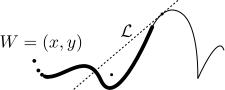
\includegraphics{puntolinea} 

}

\caption{Elipse}\label{fig:pressure1}
\end{figure}

\hypertarget{superficies-poliedricas}{%
\section{Superficies poliedricas}\label{superficies-poliedricas}}

www

\hypertarget{solidos-platuxf3nicos}{%
\subsection{Solidos platónicos}\label{solidos-platuxf3nicos}}

\hypertarget{los-prismas}{%
\subsection{Los prismas}\label{los-prismas}}

\hypertarget{superficies-de-revolucion-y-regladas}{%
\section{Superficies de revolucion y regladas}\label{superficies-de-revolucion-y-regladas}}

\hypertarget{superficies-curvas}{%
\section{Superficies curvas}\label{superficies-curvas}}

\hypertarget{cerradas}{%
\subsection{Cerradas}\label{cerradas}}

Esfera Elipsoide

\hypertarget{abiertas}{%
\subsection{Abiertas}\label{abiertas}}

\hypertarget{orientables}{%
\subsection{Orientables}\label{orientables}}

\hypertarget{no-orientables}{%
\subsection{No orientables}\label{no-orientables}}

\hypertarget{fractales-3d}{%
\section{Fractales 3D}\label{fractales-3d}}

\hypertarget{desarrollo-de-forma-tridimensionales}{%
\section{Desarrollo de forma tridimensionales}\label{desarrollo-de-forma-tridimensionales}}

\hypertarget{composiciuxf3n-de-formas}{%
\chapter{Composición de formas}\label{composiciuxf3n-de-formas}}

\hypertarget{operaciones-con-formas}{%
\section{Operaciones con formas}\label{operaciones-con-formas}}

\hypertarget{union}{%
\subsection{Union}\label{union}}

\begin{definition}
\protect\hypertarget{def:unnamed-chunk-2}{}{\label{def:unnamed-chunk-2} }wwwwwwwwwwwwwwwwwwwwwww
\end{definition}

\hypertarget{interseccion}{%
\subsection{Interseccion}\label{interseccion}}

\hypertarget{diferencia}{%
\subsection{Diferencia}\label{diferencia}}

\hypertarget{diferencia-simetrica}{%
\subsection{Diferencia simetrica}\label{diferencia-simetrica}}

\hypertarget{complemento}{%
\subsection{Complemento}\label{complemento}}

\hypertarget{componiendo-escenas}{%
\section{Componiendo escenas}\label{componiendo-escenas}}

\hypertarget{utilizando-software}{%
\subsection{Utilizando software}\label{utilizando-software}}

\hypertarget{el-bodegon}{%
\subsection{El bodegon}\label{el-bodegon}}

\hypertarget{la-superficie}{%
\subsection{La superficie}\label{la-superficie}}

\hypertarget{wwwwwwwwwww}{%
\subsection{wwwwwwwwwww}\label{wwwwwwwwwww}}

\hypertarget{simetruxedas}{%
\section{Simetrías}\label{simetruxedas}}

\hypertarget{simetruxeda-axial}{%
\subsection{Simetría axial}\label{simetruxeda-axial}}

\hypertarget{simetruxeda-radial-o-puntual}{%
\subsection{Simetría radial o puntual}\label{simetruxeda-radial-o-puntual}}

\hypertarget{simetruxeda-esferica}{%
\subsection{Simetría esferica}\label{simetruxeda-esferica}}

\hypertarget{simetruxeda-planar}{%
\subsection{Simetría planar}\label{simetruxeda-planar}}

\hypertarget{transformaciones-de-las-formas}{%
\chapter{Transformaciones de las formas}\label{transformaciones-de-las-formas}}

Una transformación en el plano es una correspondencia uno a uno entre los puntos del plano entre sí. Si un punto \(P\) se transforma en un punto \(P'\) a este último se le conoce como la imagen y a \(P\) se le llama la preimagen.

\hypertarget{transformaciones-elementales}{%
\section{Transformaciones elementales}\label{transformaciones-elementales}}

\hypertarget{traslaciuxf3n}{%
\subsection{Traslación}\label{traslaciuxf3n}}

\begin{definition}[Traslación]
\protect\hypertarget{def:traslacion}{}{\label{def:traslacion} \iffalse (Traslación) \fi{} }La traslacion de un objeto, consiste en mover todos los puntos del objeto en el espacio 2D o 3D en una solo dirección, un solo sentido y a una distancia determinada. Hay congruencia y semejanza
\end{definition}

En geometría, una \textbf{traslación} es una isometría en el espacio euclídeo caracterizada por un vector, tal que, a cada punto \(P\) de un objeto o figura se le hace corresponder otro punto \(P'\), tal que:

\[
\begin{cases}T_{\vec {u}}:\mathbb {R} ^{n}\to \mathbb {R} ^{n}&{\overrightarrow {PP'}}={\vec {u}}\\P\mapsto P'=T(P)=P+{\vec {u}}\end{cases}
\]

\begin{example}
\protect\hypertarget{exm:unnamed-chunk-3}{}{\label{exm:unnamed-chunk-3} }
\end{example}

\begin{figure}

{\centering \includegraphics[width=5.44in]{trasformacion} 

}

\caption{Hola}\label{fig:Dogewwwwww}
\end{figure}

En la escala u homotecia también existen procedimientos de proporción.

\hypertarget{rotacion}{%
\subsection{Rotacion}\label{rotacion}}

\begin{definition}[Traslación]
\protect\hypertarget{def:rotacion}{}{\label{def:rotacion} \iffalse (Traslación) \fi{} }Rotación es el movimiento de cambio de orientación de un cuerpo o un sistema de referencia de forma que una línea (llamada eje de rotación) o un punto permanece fijo.
\end{definition}

\hypertarget{reflexiuxf3n}{%
\subsection{Reflexión}\label{reflexiuxf3n}}

Sea \(\mathcal{L}\) una recta en un plano. Una reflexión sobre la recta \(\mathcal{L}\) es una transformación que proyecta cada punto \(P\) del plano sobre otro punto \(P'\) del mismo plano de manera que:

\begin{enumerate}
\def\labelenumi{\arabic{enumi}.}
\item
  Si \(P\) está en \(\mathcal{L}\), entonces \(P'=P\)
\item
  Si \(P\) no está en \(\mathcal{L}\), entonces \(\mathcal{L}\) es la mediatriz del \(\overline{PP'}\)
\end{enumerate}

\begin{remark}
\iffalse{} {Observación. } \fi{}
\end{remark}

La mediatriz de un segmento es la recta perpendicular al segmento y que pasa por el punto medio de éste.

Un segmento cuyos extremos sean los puntos \(A\) y \(B\) lo representamos como \(\overline{AB}\) y a su longitud como \(AB\). A la recta que contiene los puntos \(A\) y \(B\) la representamos como \(\overleftrightarrow{AB}\) .

Semejanza y congruencia

\hypertarget{homotecia}{%
\subsection{Homotecia}\label{homotecia}}

La homotecia es la deformación de una figura, que se hace más grande o más pequeña, todo en base a un punto el cual se toma como una referencia conocido como: \emph{centro de la homotecia}.

Semejanza

\hypertarget{trasformaciones-topoluxf3gicas}{%
\section{Trasformaciones topológicas}\label{trasformaciones-topoluxf3gicas}}

Coloquialmente, se presenta a la topología como la geometría de la página de goma (chicle). Esto hace referencia a que, en la geometría euclídea, dos objetos serán equivalentes mientras podamos transformar uno en otro mediante isometrías (rotaciones, traslaciones, reflexiones, homotescia.), es decir, mediante transformaciones que conservan las medidas de ángulo, área, longitud, volumen y otras.

\begin{definition}[Topología]
\protect\hypertarget{def:topologia}{}{\label{def:topologia} \iffalse (Topología) \fi{} }
\end{definition}

La \textbf{topología}, dedicada al estudio de aquellas propiedades de los cuerpos geométricos que permanecen inalteradas por transformaciones continuas. La topología se interesa por conceptos como \emph{proximidad}, \emph{número de agujeros}, el tipo de \emph{consistencia} (o \emph{textura}) que presenta un objeto, comparar objetos y clasificar múltiples atributos donde destacan conectividad, compacidad, metricidad o metrizabilidad, entre otros.

En topología, dos objetos son equivalentes en un sentido mucho más amplio. Han de tener el mismo número de \emph{trozos}, \emph{huecos}, \emph{intersecciones}, etc. En topología está permitido doblar, estirar, encoger, retorcer, etc., los objetos, pero siempre que se haga \emph{sin romper ni separar lo que estaba unido, ni pegar lo que estaba separado}. Por ejemplo, un triángulo es topológicamente lo mismo que una circunferencia, ya que podemos transformar uno en otra de forma continua, sin romper ni pegar. Pero una circunferencia no es lo mismo que un segmento, ya que habría que partirla (o pegarla) por algún punto.

\hypertarget{isomorfismo}{%
\subsection{Isomorfismo}\label{isomorfismo}}

En matemáticas, un \textbf{isomorfismo} (del griego iso-morfos: Igual forma) es un homomorfismo (o más generalmente un morfismo) que admite un inverso. El concepto matemático de \textbf{isomorfismo} pretende captar la idea de tener la misma estructura.

\hypertarget{isometruxeda}{%
\subsection{Isometría}\label{isometruxeda}}

Una \textbf{isometría} es una trasformacion entre dos espacios métricos que conserva las distancias entre los puntos. Dado un espacio euclídeo de dos o tres dimensiones, dos figuras u objetos se dice que existe \textbf{isometría} cuando son congruentes entre sí, o viceversa.

\hypertarget{formas-naturales}{%
\chapter{Formas naturales}\label{formas-naturales}}

Son formas que están presentes en la naturaleza tales como nubes arboles, animales, cosas en general.

\begin{definition}[Formas naturales]
\protect\hypertarget{def:formasnaturales}{}{\label{def:formasnaturales} \iffalse (Formas naturales) \fi{} }Son objetos presentes en la naturaleza manisfestandose como elementos que interactuan en nuestro entorno.
\end{definition}

\hypertarget{geometrizaciuxf3n}{%
\section{Geometrización}\label{geometrizaciuxf3n}}

La geometrización es el proceso de manifestar poligonos y lineas sobre los objetos naturales 2d y 3d. Este proceso es la simplificación del objeto con el objetivo de poder aplicar criterios de proporcionalidad y otras trasformaciones elementales que puedan realizarse sobre el objeto. La simplificación podría incluso ser una linea o una estructura poligonal compleja. La geometrización se realiza desde un punto de vista especifico en el caso bidimensional y toda la forma en el caso tridimensional.

El objetivo es aprender a geometrizar diversos objetos 3d con el objetivo de trasformarlos.

\begin{figure}[!ht]

{\centering \includegraphics{geometrizacion} 

}

\caption{Elipse}\label{fig:geometrizacion-1}
\end{figure}
\begin{figure}[!ht]

{\centering \includegraphics[width=3.12in]{images} 

}

\caption{Elipse}\label{fig:geometrizacion-2}
\end{figure}
\begin{figure}[!ht]

{\centering \includegraphics{pol1} 

}

\caption{Elipse}\label{fig:geometrizacion-3}
\end{figure}
\begin{figure}[!ht]

{\centering \includegraphics{pol2} 

}

\caption{Elipse}\label{fig:geometrizacion-4}
\end{figure}

\hypertarget{geomorfologia}{%
\section{Geomorfologia}\label{geomorfologia}}

\begin{definition}[Geomorfología]
\protect\hypertarget{def:www2}{}{\label{def:www2} \iffalse (Geomorfología) \fi{} }La geomorfología es una rama de la geografía1 y de la geología que tiene como objetivo el estudio de las formas de la superficie terrestre enfocado en describir, entender su génesis y su actual comportamiento.
\end{definition}
La geomorfología es una rama de la geografía y de la geología que tiene como objetivo el estudio de las formas de la superficie terrestre enfocado en describir, entender su génesis y su actual comportamiento.

\hypertarget{factores-generadores-de-los-procesos-geomorfoluxf3gicos}{%
\subsection{Factores generadores de los procesos geomorfológicos}\label{factores-generadores-de-los-procesos-geomorfoluxf3gicos}}

\begin{itemize}
\tightlist
\item
  \textbf{Factores geográficos:} Factores \emph{bióticos} como \emph{abióticos}, son propiamente geográficos aquellos \emph{abióticos} de origen exógeno, tales como la \emph{gravedad}, el suelo, el clima y los cuerpos de agua. El clima con sus elementos tales como la \emph{presión}, la \emph{temperatura}, la \emph{humedad}, los vientos. El \emph{agua superficial}. Son factores que ayudan al modelado, favoreciendo los procesos erosivos.
\item
  \textbf{Factores bióticos}
\item
  \textbf{Factores geológicos:} Tales como la tectónica, el diastrofismo, la orogénesis y el vulcanismo, son procesos constructivos y de origen endógeno que se oponen al modelado e interrumpen el ciclo geográfico
\item
  \textbf{Factores antrópicos}
\end{itemize}

\hypertarget{ramas-de-la-geomorfologuxeda}{%
\subsection{Ramas de la geomorfología}\label{ramas-de-la-geomorfologuxeda}}

\begin{itemize}
\item
  \textbf{Geomorfología climática}: Estudia la influencia del clima en el desarrollo del relieve. La presión atmosférica y la temperatura interactúan con el clima y son los responsables de los vientos, las escorrentías y del continuo modelado del ciclo geográfico. La diversidad de climas representa distintas de velocidades en la evolución del ciclo, como es el caso de los climas áridos con ritmo evolutivo más lentos y de los climas muy húmedos con ritmos evolutivos más altos, como también el clima representa el tipo de modelado predominante; glacial, eólico, fluvial, etc. Este conocimiento se sintetiza en lo que se denomina «dominios morfoclimáticos.
\item
  \textbf{Geomorfología fluvial}: Estudio de formas y relieves ocasionados por la dinámica fluvial. \textasciitilde{} hidrografía.
\item
  \textbf{Geomorfología de laderas}: Estudia los fenómenos producidos en las vertientes de las montañas, movimientos en masa, estabilización de taludes, etc. riesgos naturales.
\item
  \textbf{Geomorfología eólica}: Estudiar los procesos y las formas de origen eólico, en las zonas litorales, los desiertos fríos y cálidos, y las zonas polares.
\item
  \textbf{Geomorfología glaciar}: se encarga de estudiar las formaciones y los procesos de los accidentes geográficos, formas y relieves glaciares y periglaciares. Esta rama está íntimamente ligada con la glaciología.
\item
  \textbf{Geomorfología estructural}: Prioriza la influencia de estructuras geológicas en el desarrollo del relieve. Esta disciplina es muy relevante en zonas de marcada actividad geológica donde por ejemplo fallas y plegamientos predeterminan la existencia de cumbres o quebradas, o la existencia de bahías y cabos se explica por la erosión diferencial de afloramientos de roca más o menos resistentes. geología
\item
  \textbf{Geomorfología litoral}: estudia las formas del relieve propias de las zonas costeras.
\end{itemize}

\begin{figure}[!ht]

{\centering \includegraphics{geomorfo} 

}

\caption{WWWWWWWWW}\label{fig:wwUUU}
\end{figure}

\href{https://sketchfab.com/3d-models/eldgos-i-geldingadolum-a-reykjanesskaga-7bcb3d856e1947a4a78c1810f559b3ea}{Geomorfologia 1}

Wariewood Outfall 12/01/2017 by chrisdrummond on Sketchfab

\hypertarget{fitomorfologia}{%
\section{Fitomorfologia}\label{fitomorfologia}}

\begin{definition}[Formas naturales]
\protect\hypertarget{def:ww3}{}{\label{def:ww3} \iffalse (Formas naturales) \fi{} }La Fitomorfologia, en sentido amplio, se define como el estudio de la estructura y forma de las plantas, e incluye la Citología y la Histología. La primera se ocupa del estudio fino de la constitución de la célula y la segunda del estudio de los tejidos. Citología e Histología, conjuntamente, son necesarias para comprender la anatomía vegetal, o sea, su constitución interna y, además, son un complemento de la organografía, exomorfología o morfología en sentido estricto, que trata de la forma externa de las plantas
\end{definition}
La Morfología vegetal, en sentido amplio, se define como el estudio de la \textbf{estructura} y forma de las plantas, e incluye la Citología y la Histología. La primera se ocupa del estudio fino de la constitución de la célula y la segunda del estudio de los tejidos. Citología e Histología, conjuntamente, son necesarias para comprender la anatomía vegetal, o sea, su constitución interna y, además, son un complemento de la organografía, \textbf{exomorfología} o morfología en sentido estricto, que trata de la forma externa de las plantas

\hypertarget{metodos}{%
\subsection{Metodos}\label{metodos}}

Las plantas nos ofrecen una infinidad de formas particulares y el objetivo de la morfología es descubrir los patrones o regularidades generales en el fondo de tal diversidad, asimismo comprender y describir tal diversidad desde varios puntos de vista. Para alcanzar este fin se pueden seguir dos caminos:

\begin{itemize}
\item
  Secuencias
\item
  Morfogenesis
\end{itemize}

\hypertarget{organizaciuxf3n-del-cuerpo-de-la-planta}{%
\subsection{Organización del cuerpo de la planta}\label{organizaciuxf3n-del-cuerpo-de-la-planta}}

El cuerpo de las plantas vasculares está marcadamente polarizado y formado por dos porciones básicas: un vástago orientado hacia la luz, que vive en ambiente aéreo, compuesto por tallo y hojas, y una raíz, órgano de fijación y absorción que vive en el suelo. Este tipo de cuerpo vegetativo se llama cormo y se presenta en las pteridófitas y en las espermatófitas, que por eso se llaman también cormófitos.

Es difícil hacer una distinción entre tallo y hojas, ambos órganos tienen origen común en el meristema apical caulinar, y están relacionados con estrecha dependencia a lo largo de todo su período de crecimiento. Por eso tallo y hojas se consideran como una unidad que constituye el vástago.

En las espermatófitas la diferenciación entre raíz y vástago aparece ya en el embrión joven. Las partes del embrión son radícula, hipocótilo, cotiledones y plúmula. En algunos casos se distingue también el primer entrenudo, entre el nudo cotiledonar y la plúmula: el epicótilo. Durante la germinación el embrión crece, la radícula formará la raíz primaria y la plúmula formará el vástago.

\hypertarget{zoomorfologia}{%
\section{Zoomorfologia}\label{zoomorfologia}}

\emph{Keywords}: Metamorfosis, locomocion, simetria, equilibrio, secuencias unidad, variedad, anatomia (esquelética y muscular)

\textbf{Locomocion} El concepto alude al traslado de un sitio a otro. La locomoción, por lo tanto, es el desplazamiento físico.

\textbf{Metamorfosis} Se llama metamorfosis a un proceso biológico por el cual un animal se desarrolla desde su nacimiento (pasado el desarrollo embrionario) hasta la madurez por medio de grandes cambios estructurales y fisiológicos

\textbf{Anatomia} La anatomía es una ciencia que estudia la estructura de los seres vivos, es decir, la forma, topografía, la ubicación, la disposición y la relación entre sí de los órganos que las componen.

Animales estructura muscular y osea locomoción

\hypertarget{formas-abstractas}{%
\chapter{Formas abstractas}\label{formas-abstractas}}

wwwwwwwwwwwwwwwwwwwwwwwwwww

\hypertarget{funciones}{%
\section{Funciones}\label{funciones}}

wwwwwwwwww\index{wwwwwwww} \citep{vincze2014college}

\hypertarget{ejercicios}{%
\section{Ejercicios}\label{ejercicios}}

\hypertarget{appendix-apendice}{%
\appendix \addcontentsline{toc}{chapter}{\appendixname}}


Temas de reforzamiento o conocimientos preliminares que son necesarias para entender el contenido.

\hypertarget{trasformaciones}{%
\chapter{Trasformaciones}\label{trasformaciones}}

Se refiere a las transformaciones o modificaciones que pueden sufrir las formas, es decir los achatamientos, las elongaciones los cambios de posición etc., mediante la manipulación de los puntos pertenecientes a la forma.

\begin{definition}[Transformación]
\protect\hypertarget{def:transformacion}{}{\label{def:transformacion} \iffalse (Transformación) \fi{} }Una transformacion es el proceso de modificar una forma covirtiendola en otra
\end{definition}

\hypertarget{trasformaciones-elementales}{%
\section{Trasformaciones elementales}\label{trasformaciones-elementales}}

En esta sección se trata sobre la trasformaciones básicas que son la traslación, la rotación, la reflexión y la homotescia o escala

\hypertarget{centro-de-masa}{%
\chapter{Centro de masa}\label{centro-de-masa}}

\hypertarget{centro-de-masa-de-objetos-2d}{%
\section{Centro de masa de objetos 2D}\label{centro-de-masa-de-objetos-2d}}

\hypertarget{metodos-matematicos}{%
\subsection{Metodos matematicos}\label{metodos-matematicos}}

\hypertarget{metodos-tecnicos}{%
\subsection{Metodos tecnicos}\label{metodos-tecnicos}}

\hypertarget{muxe9todo-del-borde-de-la-mesa}{%
\subsubsection{Método del borde de la mesa}\label{muxe9todo-del-borde-de-la-mesa}}

\hypertarget{muxe9todo-de-la-plomada}{%
\subsubsection{Método de la plomada}\label{muxe9todo-de-la-plomada}}

\hypertarget{centro-de-masa-de-objetos-3d}{%
\section{Centro de masa de objetos 3D}\label{centro-de-masa-de-objetos-3d}}

\hypertarget{metodos-matematicos-1}{%
\subsection{Metodos matematicos}\label{metodos-matematicos-1}}

\hypertarget{metodos-tecnicos-1}{%
\subsection{Metodos tecnicos}\label{metodos-tecnicos-1}}

\hypertarget{muxe9todo-de-las-secciones}{%
\subsubsection{Método de las secciones}\label{muxe9todo-de-las-secciones}}

\hypertarget{muxe9todo-de-la-plomada-1}{%
\subsubsection{Método de la plomada}\label{muxe9todo-de-la-plomada-1}}

\bibliography{book.bib,packages.bib}

\printindex

\end{document}
